% Document Class and packages
\documentclass[a4paper, 12pt]{memoir}
\usepackage{subfiles}
\usepackage[utf8]{inputenc}
\usepackage[italian]{babel}
\usepackage{graphicx}
\usepackage[usenames,dvipsnames,svgnames,table]{xcolor}
\usepackage{geometry}
\usepackage{cite}

% Increase space between paragraphs
\setlength{\parskip}{3pt}

% about:author
\author{Paolo Scaramuzza}
\title{Studio dell' efficienza di oscillatori LC integrati per impulsatori 
	Ultra Wideband}
\date{} % HACK: avoids date in the title

\begin{document}
\subfile{tex/front} % make a nice front page (thanks HammondSmoking)

%%%%%%%%%%%%%%%%%%%%%%%%%%%%%
% Abstract
%%%%%%%%%%%%%%%%%%%%%%%%%%%%%
\cleardoublepage{}
\newpage
\pagenumbering{gobble} % no need for numbering
\begin{vplace}[0.7]
	\subfile{tex/abstract}
\end{vplace}
%%%%%%%%%%%%%%%%%%%%%%%%%%%%%
% Index
%%%%%%%%%%%%%%%%%%%%%%%%%%%%%
\cleardoublepage{}
\newpage
\tableofcontents

\pagenumbering{arabic} % restore normal page numbering
%%%%%%%%%%%%%%%%%%%%%%%%%%%%%
% Introduzione
%%%%%%%%%%%%%%%%%%%%%%%%%%%%%
\cleardoublepage{}
\chapter{Introduzione}
Contrariamente a molte tecnologie in radiofrequenza oggi in uso, la radio a
impulsi Ultra-Wideband (\emph{Ultra-Wideband Impulse-Radio}, UWB IR)
sfrutta un' ampia porzione dello spettro delle radiofrequenze (di ampiezza
maggiore a 500MHz oppure più del 25\% della frequenza di centro-banda
\cite{Neviani12}) trasmettendo i dati sotto forma di impulsi di breve durata.\\
Tra gli schemi di modulazione impiegati si trovano: 
\begin{itemize}
	\item \emph{on-off keyng} (OOK)
	\item \emph{pulse-position modulation} (PPM)
\end{itemize}

Per molti anni la UWB IR è stata impiegata esclusivamente in ambito
militare. Nel 2002, con la regolamentazione dello spettro di frequenze tra 3.1 
e 10.6GHz da parte degli Stati Uniti e in seguito dall'Europa e dal Giappone,
la radio UWB ha iniziato ad affermarsi quale soluzione più conveniente, sia dal
punto di vista economico che prestazionale, per la comunicazione a corto raggio.
\\La massima densità spettrale di potenza in trasmissione consentita dalle
leggi europee è di $ -41.3 dBm/MHz $ e in alcuni segmenti dello spettro tale
limite può arrivare fino a $ -75 dBm/MHz $, come evidenziato in\cite{Hirt07}.\\
Vista la bassa potenza di trasmissione e le elevate frequenze operative,
le radio a impulsi UWB ben si prestano ad essere realizzate interamente in
tecnologia CMOS.\@
Si possono avere così trasmettitore e ricevitore in un unico circuito integrato.
\\Tra le possibili applicazioni di questa tecnologia si trovano: la
localizzazione di precisione e la trasmissione a corto raggio.

Per la localizzazione si cita\cite{Terada05} in cui si mostra una radio 
Ultra-Wideband realizzata in tecnologia CMOS da $ 180nm $ in grado di
effettuare localizzazioni a più di un metro di distanza con un errore massimo
di $ \pm 2.5cm $.
Quando si effettuano mille misurazioni al secondo il consumo di potenza è pari
a $ 0.7\mu W $. Il trasmettitore e il ricevitore sono integrati in un unico
chip avente un' area di $ 0.415mm^2 $.

Per la trasmissione a corto raggio significativi risultati sono stati raggiunti
da\cite{RabaeyEECS},\cite{Neviani12} e\cite{Gambini12} in cui sono dimostrate
varie soluzioni circuitali che permettono di ottenere, in un unico circuito
integrato di piccole dimensioni, sia la funzionalità di trasmettitore che di
ricevitore.

Attualmente la frontiera della ricerca si sta spostando verso una sempre
maggiore integrazione e un miglioramento globale dell'efficienza energetica.
Questi risultati della Ricerca permettono di avere radio dalla durata della 
batteria estremamente lunga o di far funzionare la circuiteria tramite
\emph{energy harvesting}.\\
Un esempio significativo è\cite{Danesh11} in cui si ha un nodo sensore 
alimentato da un pannello solare di $ 2\times2 cm^2 $ che svolge anche la
funzione di antenna. Il sensore è poco più grande del pannello solare, consuma
solamente $ 10\mu W $ di potenza e trasmette i dati a intervalli di un
minuto alla velocità di $ 1 KB/s $ tramite la modulazione \emph{on-off
keying}.
Con l' impiego di un supercondensatore, inoltre, è in grado di lavorare in
condizioni di totale assenza di illuminazione per più di due giorni.\\
In\cite{Solda10} infine è dimostrata la realizzazione di una radio a impulsi 
che garantisce un' efficienza in trasmissione pari al 7\% mentre in 
\cite{Neviani14} si raggiunge l' 11,7\%, valore che rappresenta l' attuale
stato dell'arte.

La presente tesi parte proprio dai risultati ottenuti in~\cite{Neviani12} e
\cite{Neviani14} e mira a massimizzare l'efficienza energetica dell'oscillatore
LC \emph{cross-coupled} in uso nell'impulsatore.

In Figura 1.1 è rappresentato lo schema elettrico di un oscillatore LC
\emph{cross coupled} nella sua forma più semplice.\\
\begin{figure}[h]
\centering
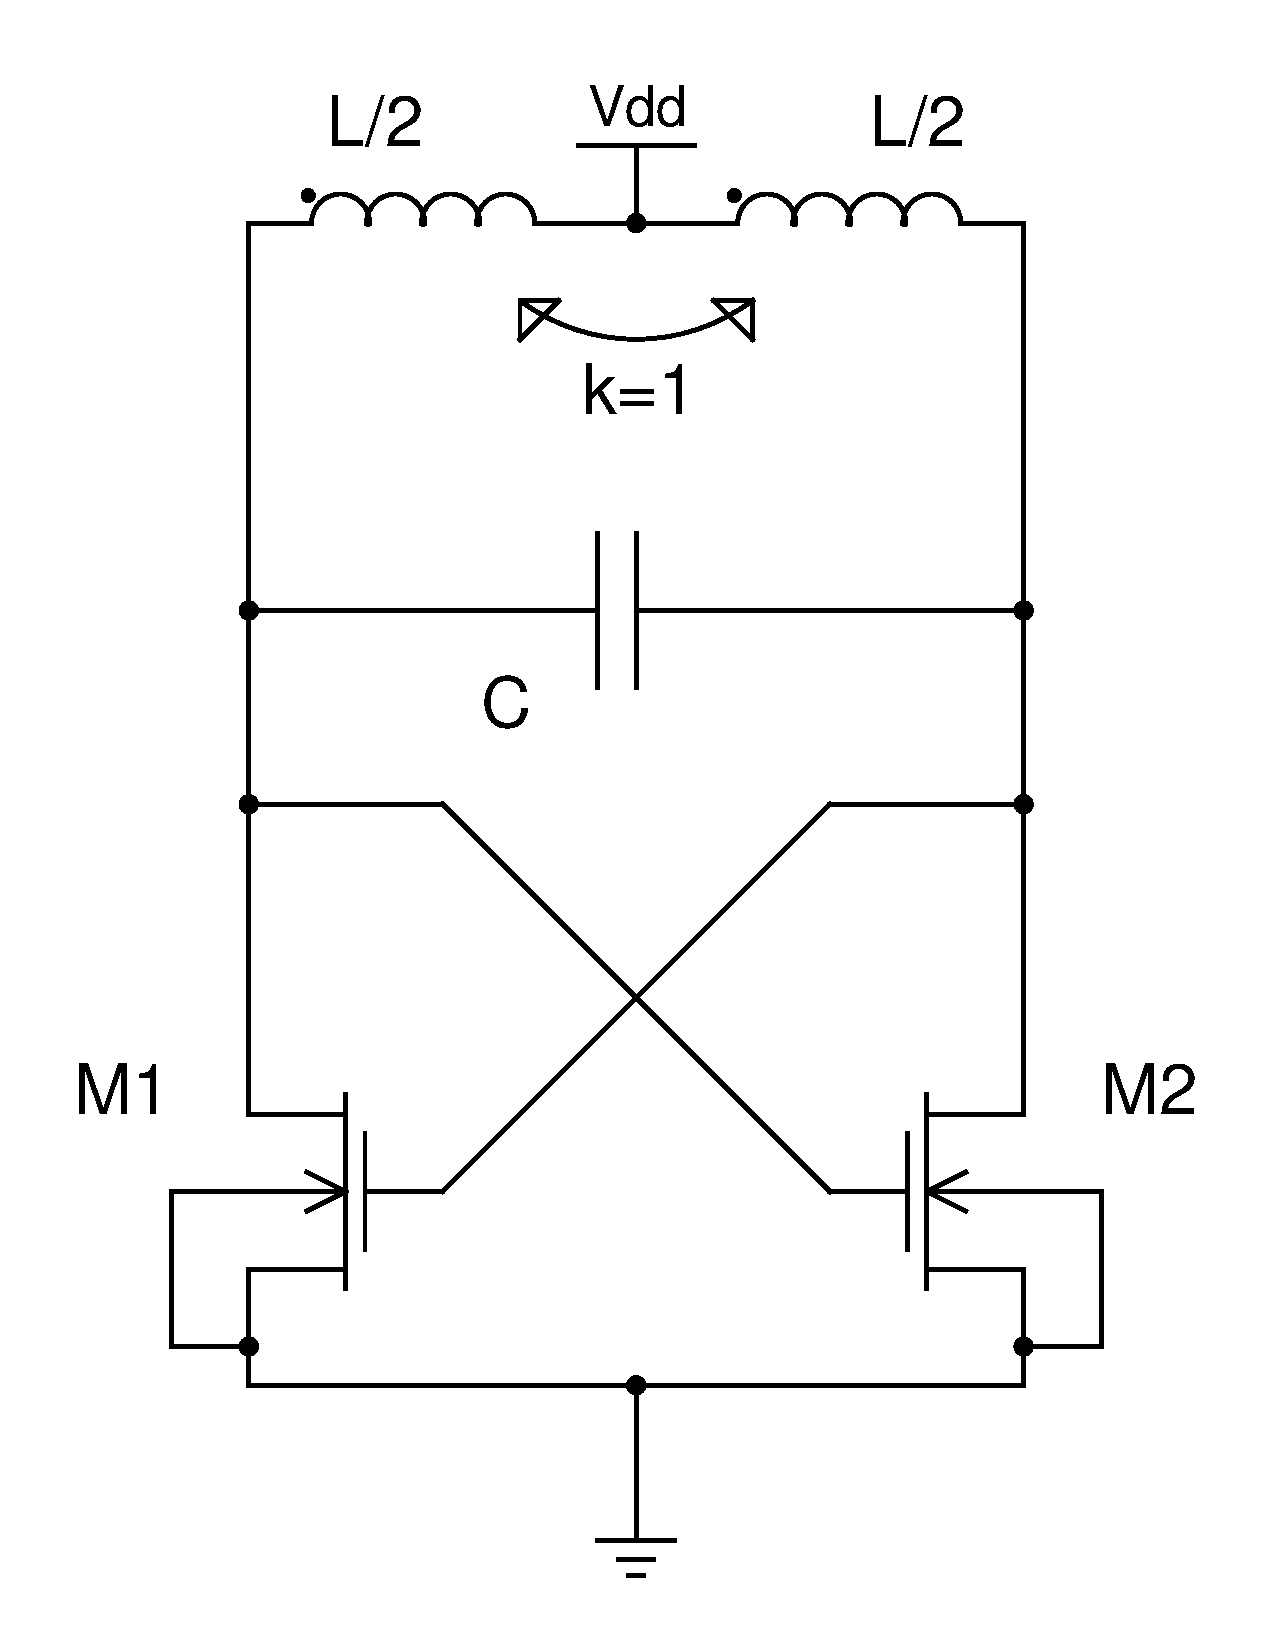
\includegraphics[width=0.34\textwidth]{images/LCosc.pdf}
\caption{Schema elettrico dell'oscillatore LC \emph{cross-coupled}}
\end{figure}
\`E la tipologia di oscillatore più diffusa nei circuiti integrati perché il
rumore di fase è più basso rispetto ad altre soluzioni e richiede un basso
numero di componenti attivi\cite{Amran05}.

Il suo funzionamento si basa sulla risonanza tra l'induttanza e la capacità
presenti nel circuito. \\
Gli NMOS del circuito infatti formano una coppia incrociata e ognuno dei due
rami apporta, come si evince dai diagrammi di Bode in Figura 1.2, uno
sfasamento di $ 180^{\circ} $ alla pulsazione $ \omega _r=\frac{1}{\sqrt{LC}} $.

Per il singolo ramo del circuito, detta $ R_p $ la resistenza parassita
complessiva e $ g_m $ la transconduttanza del MOSFET, si ha la seguente
funzione di trasferimento:
\begin{center}
$ W(s)=\frac{V_{out}}{V_{in}}=-g_m Z(s)=-g_m \frac{R_p L s}{R_p C L s^2 + Ls + R_p} $
\end{center}

\begin{figure}[h]
\centering
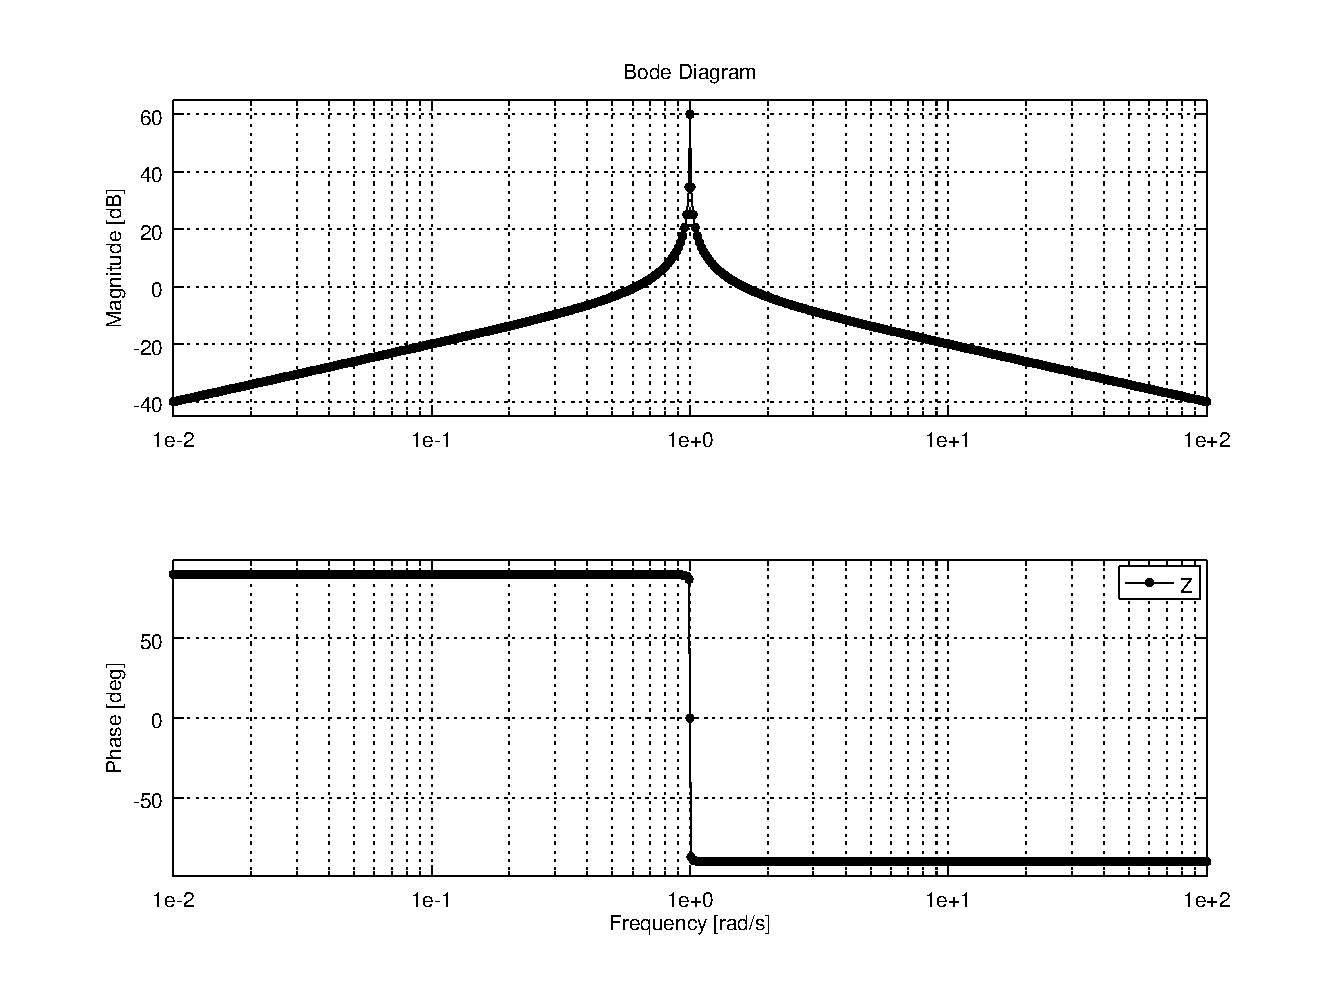
\includegraphics[width=\textwidth]{images/BodeLC.pdf}
\caption{Diagramma di Bode per $ Z(s) $ con $L=1H$, $C=1F$ e $R_p=1K\Omega$}
\end{figure}

In considerazione della $ W(s) $ sopra descritta è possibile applicare il
criterio di Barkhausen\cite{JaegerMicro} che afferma che il circuito si
comporta da oscillatore se alla pulsazione $ \omega _r $ il modulo della
funzione di trasferimento in catena aperta è pari ad uno e lo sfasamento è di
$ 360^{\circ} $.\\
Per avere oscillazione è dunque necessario porre in cascata, chiudendo l'
anello di retroazione, due stadi del tipo di circuito presentato in Figura 1.3,
assicurandosi che $ {\left( g_m R_p \right)}^2 = 1 $ 
\cite[p.652]{RazaviFundamentals}.\\
Riorganizzando lo schema circuitale si riottiene quello in Figura 1.1.

\begin{figure}[h]
\centering
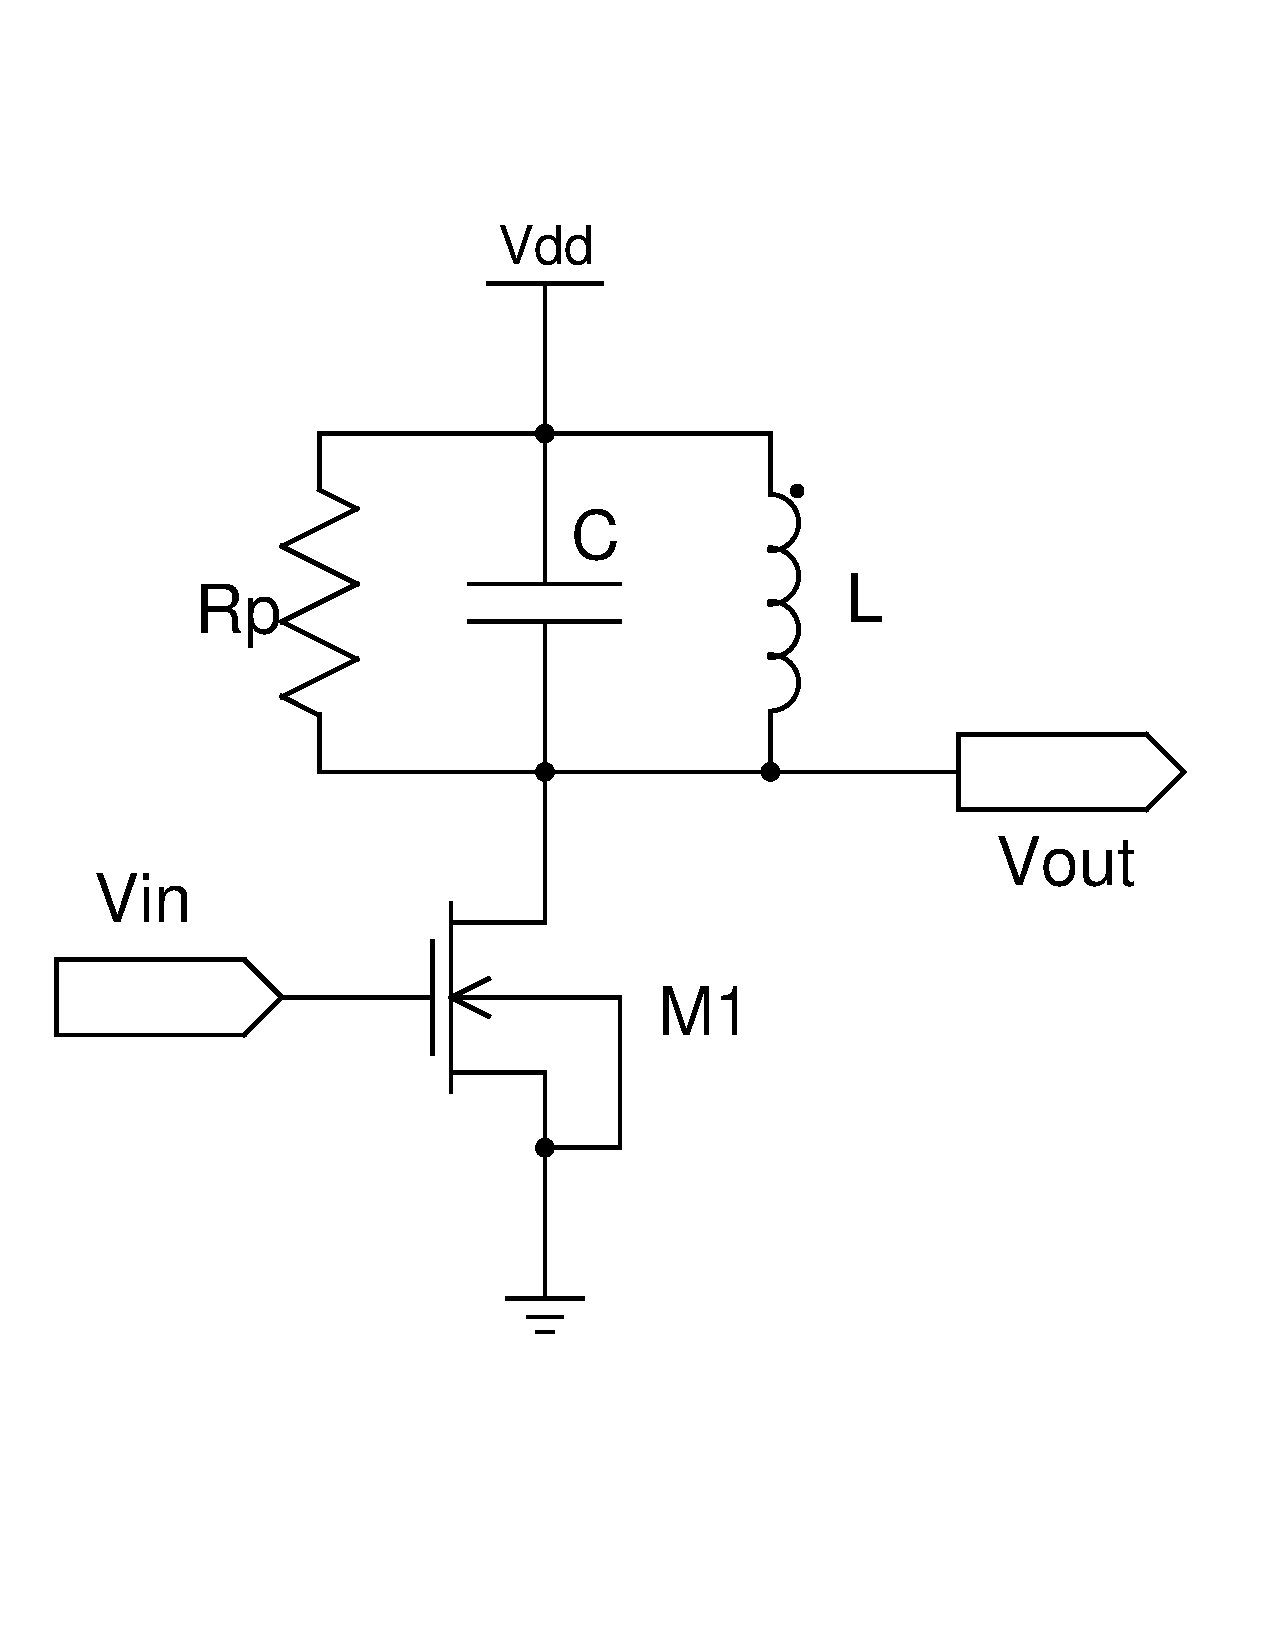
\includegraphics[width=0.4\textwidth]{images/LCsingle.pdf}
\caption{Schema per il singolo ramo dell'oscillatore}
\end{figure}

\section{Contributi della tesi}
Nell'ambito del lavoro svolto i valori dell'induttanza e della capacità sono
tarati in modo tale da produrre un' onda sinusoidale alla frequenza di 8GHz.\\
L' induttanza è sostituita da un trasformatore al cui secondario è collegata l'
antenna. La circuiteria di controllo aggiunta si occupa di attivare e
disattivare l' oscillatore per produrre gli impulsi.

Un modello teorico semplificato per il circuito è stato ricavato approssimando
i MOSFET come dei generatori ideali di tensione alternata ad 8GHz
connessi al primario del trasformatore. \\
Tale modello ha permesso di valutare in prima approssimazione l' effetto sul
comportamento del circuito delle variazioni nel dimensionamento dei componenti.

Partendo dai valori ottenuti in\cite{Neviani14} si è poi effettuata la
simulazione al calcolatore del circuito a livello di transistor.\\
Si è evidenziato che, a meno di effetti di ordini successivi al primo, i
risultati della simulazione sono in accordo con il modello teorico.\\
Affinando le indicazioni del modello tramite il calcolatore, si sono
raggiunti valori di efficienza massima per il circuito simulato nell'intorno
del 29\%, partendo da un valore iniziale pari al 10\%.\\
Le simulazioni effettuate su trasformatore da solo confermano ulteriormente i
risultati ottenuti.

Si presentano e discutono infine i massimi valori di efficienza raggiunti nelle
simulazioni dalle due topologie ed è illustrato come queste differiscano poco l'
una dall'altra dal punto di vista dell'efficienza. \\
La scelta di un tipo di oscillatore piuttosto che l' altro deve dunque essere
dettata da altri parametri (ad esempio l' occupazione di area ed il consumo
dinamico di potenza) che esulano dal contributo di questa tesi e sono solo
accennati.

\section{Struttura dell'elaborato}
Il presente elaborato è organizzato come segue:
\begin{itemize}
\item Nel Capitolo 2 sono presentate le due diverse tipologie di oscillatore
	prese in esame. \`E discusso come da essi si giunga ad un modello
	semplificato e si presenta un'analisi qualitativa degli effetti
	sull'efficienza del diverso dimensionamento dei componenti nel
	modello ottenuto
\item Nel Capitolo 3 sono presentati e discussi i risultati numerici delle
	simulazioni, confrontando le diverse topologie dell'oscillatore
\item Il Capitolo 4 è dedicato agli sviluppi futuri e alla discussione dei
	parametri di interesse la cui valutazione si presta ad ulteriori studi.
\end{itemize}
%%%%%%%%%%%%%%%%%%%%%%%%%%%%%
% Tipologie e parametri
%%%%%%%%%%%%%%%%%%%%%%%%%%%%%
\cleardoublepage{}
\chapter{Topologie e parametri di interesse}
\cite{RazaviRF}

%%%%%%%%%%%%%%%%%%%%%%%%%%%%%
% Risultati numerici
%%%%%%%%%%%%%%%%%%%%%%%%%%%%%
\cleardoublepage{}
\chapter{Risultati numerici}
\includegraphics[width=\textwidth]{efficienza.pdf}

%%%%%%%%%%%%%%%%%%%%%%%%%%%%%
% Conclusione e sviluppi futuri
%%%%%%%%%%%%%%%%%%%%%%%%%%%%%
\cleardoublepage{}
\chapter{Conclusione}

\section{Sviluppi futuri}

%%%%%%%%%%%%%%%%%%%%%%%%%%%%%
% Bibliografia
%%%%%%%%%%%%%%%%%%%%%%%%%%%%%
\bibliographystyle{plain}
\bibliography{tex/biblio}
\end{document}
